\documentclass[12pt]{article}

\usepackage{fullpage}
\usepackage{graphicx}
\usepackage{amssymb}
\usepackage{amsmath}
\usepackage[none]{hyphenat}
\usepackage{parskip}
\usepackage[spanish]{babel}
\usepackage[utf8]{inputenc}
\usepackage{hyperref}
\usepackage{fancyhdr}
\usepackage{tasks}
\usepackage{mdframed}
\usepackage{xcolor}
\usepackage{pgfplots}
\usepackage[makeroom]{cancel}
\usepackage{multicol}
\usepackage[shortlabels]{enumitem}
\usepackage{stackrel}
\usepackage{tkz-tab}
\usepackage{xpatch}
\usepackage{tkz-euclide}
\usetkzobj{all}
\usepackage{tabto}
\xpatchcmd{\tkzTabLine}{$0$}{$\bullet$}{}{}

\setlength{\headheight}{10pt}
\setlength{\headsep}{10pt}
\pagestyle{fancy}
\rhead{\ayudantia \ - \alumno}
\tikzset{t style/.style={style=solid}}

\newcommand*{\mybox}[2]{\colorbox{#1!30}{\parbox{.98\linewidth}{#2}}}

\newenvironment{solucion}
{\begin{mdframed}[backgroundcolor=black!10]
		{\bf Solución:}\\
	}
	{
	\end{mdframed}
}

\newenvironment{alternativas}[1]
{\begin{multicols}{#1}
		\begin{enumerate}[a)]
		}
		{
		\end{enumerate}
	\end{multicols}
}

\newenvironment{preguntas}
{\begin{enumerate}\itemsep12pt
	}
	{
	\end{enumerate}
}

\newcommand{\ayudantia}{{\sc Ayudantía 9.5}}
\newcommand{\tituloayu}{Compilado I2}
\newcommand{\fecha}{9 de noviembre de 2019}
\newcommand{\sigla}{MAT210E}
\newcommand{\nombre}{Cálculo I}
\newcommand{\profesor}{Claudio Fernandez}
\newcommand{\ano}{2016}
\newcommand{\semestre}{1}
\newcommand{\mail}{mat210e@ifcastaneda.cl}
\newcommand{\alumno}{Ignacio Castañeda - \mail}

\newcommand{\ev}{\Big|}
\newcommand{\ra}{\rightarrow}
\newcommand{\lra}{\leftrightarrow}
\newcommand{\N}{\mathbb{N}}
\newcommand{\R}{\mathbb{R}}
\newcommand{\Exp}[1]{\mathcal{E}_{#1}}
\newcommand{\List}[1]{\mathcal{L}_{#1}}
\newcommand{\EN}{\Exp{\N}}
\newcommand{\LN}{\List{\N}}
\newcommand{\comment}[1]{}
\newcommand{\lb}{\\~\\}
\newcommand{\eop}{_{\square}}
\newcommand{\hsig}{\hat{\sigma}}
\newcommand{\widesim}[2][1.5]{
	\mathrel{\overset{#2}{\scalebox{#1}[1]{$\sim$}}}
}
\newcommand{\wsim}{\widesim{}}
\newcommand{\lh}{\stackrel{L'H}{=}}

\begin{document}
\thispagestyle{empty}

\begin{minipage}{2cm}
	
\includegraphics[width=2cm]{../../../../img/logo.pdf}
	\vspace{0.5cm}
\end{minipage}
\begin{minipage}{\linewidth}
	\begin{tabular}{lrl}
		{\scriptsize\sc Pontificia Universidad Catolica de Chile} & \hspace*{0.7in}Curso: &
		\sigla  - \nombre\\
		{\sc Facultad de Matemáticas}&
		Profesor: & \profesor \\
		{\sc Semestre \ano-\semestre} & Ayudante: & {Ignacio Castañeda}\\
		& {Mail:} & \texttt{\mail}
	\end{tabular}
\end{minipage}

\vspace{-10mm}
\begin{center}
	{\LARGE\bf \ayudantia}\\
	\vspace{0.1cm}
	{\tituloayu}\\
	\vspace{0.1cm}
	\fecha\\
	\vspace{0.4cm}
\end{center}

\begin{preguntas}
\item Determina si la siguiente serie converge o diverge
$$\sum\limits_{n=1}^{\infty}\dfrac{n!}{n^n}$$
\begin{solucion}
\begin{center}
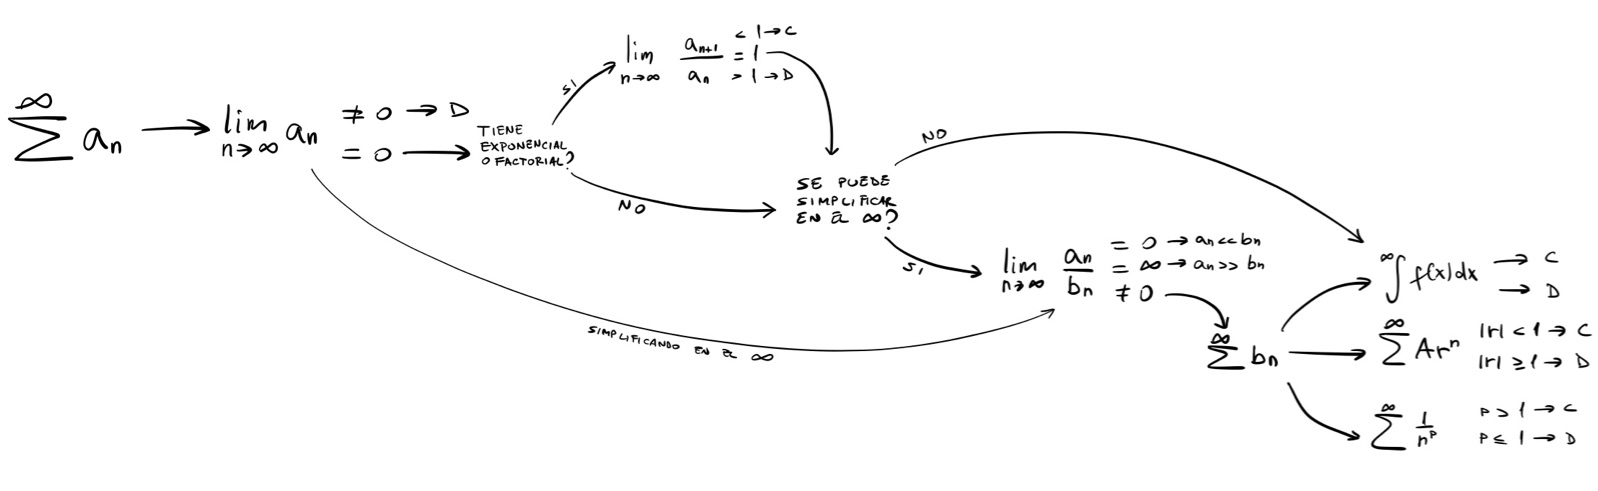
\includegraphics[width=12cm]{../../../../img/mapa_series}
\end{center}
Recordemos que en el infinito,
			$$n^n > n! > a^n > n^a > ln(n)$$
			El límite de la sucesión es
			$$\lim\limits_{n\ra\infty}\dfrac{n!}{n^n} = 0$$
			Usando el criterio de la razón,
			$$\lim\limits_{n \ra \infty} \dfrac{a_{n+1}}{a_n}
			= \lim\limits_{n \ra \infty} \dfrac{\dfrac{(n+1)!}{(n+1)^{n+1}}}{\dfrac{n!}{n^n}}
			= \lim\limits_{n \ra \infty} \dfrac{(n+1)!}{n!}\dfrac{n^n}{(n+1)^{n+1}}$$
			$$= \lim\limits_{n \ra \infty} \dfrac{(n+1)}{1}\dfrac{n^n}{(n+1)^{n+1}}
			= \lim\limits_{n \ra \infty} \dfrac{n^n}{(n+1)^{n}}
			= \lim\limits_{n \ra \infty} \left(\dfrac{n}{n+1}\right)^n$$
			$$= \lim\limits_{n \ra \infty} \dfrac{1}{\left(\dfrac{n+1}{n}\right)^n}
			= \dfrac{1}{e} < 1$$
			Por criterio de la razón, la serie es convergente.
\end{solucion}
\item Determine si las siguientes series convergen condicionalmente, absolutamente o divergen.
\begin{tasks}(3)
\task $\sum\limits_{n=1}^{\infty}\dfrac{(-1)^{n+1}}{\sqrt[]{n}}$
\task $\sum\limits_{n=2}^{\infty}\dfrac{(-1)^{n-1}(2n-1)}{(\sqrt[]{2})^n}$
\task $\sum\limits_{n=2}^{\infty}\dfrac{(-1)^{n-1}(n+1)}{n}$
\end{tasks}
\begin{solucion}

\begin{enumerate}[a)]
\item $\sum\limits_{n=1}^{\infty}\dfrac{(-1)^{n+1}}{\sqrt[]{n}}$\\
			\\
			Veamos el límite de la sucesión,
			$$\lim_{n\ra\infty} |a_n| = \lim_{n\ra\infty} \dfrac{1}{\sqrt[]{n}} = 0$$
			Además, notemos que 
			$$\dfrac{1}{\sqrt[]{n}} > \dfrac{1}{\sqrt[]{n+1}} \ra \dfrac{1}{n} > \dfrac{1}{n+1} \ra n < n+1$$
			Por lo que la sucesión es decreciente.\\
			\\
			Dicho esto, por el criterio de Leibniz, la serie converge.\\
			\\
			Veamos ahora que pasa con la serie no alternante 
			$$\sum\limits_{n=1}^{\infty}\dfrac{1}{\sqrt[]{n}} = \sum\limits_{n=1}^{\infty}\dfrac{1}{n^{1/2}}$$
			Es una serie-p con $p<1$, por lo que es divergente.\\
			\\
			Finalmente, la serie converge condicionalmente.
\item $\sum\limits_{n=2}^{\infty}\dfrac{(-1)^{n-1}(2n-1)}{(\sqrt[]{2})^n}$\\
			\\
			Veamos el límite de la sucesión,
			$$\lim_{n\ra\infty} |a_n| = \lim_{n\ra\infty} \dfrac{2n-1}{(\sqrt[]{2})^n} = 0$$
			Usando el criterio de la razón,
			$$\lim\limits_{n \ra \infty} \left|\dfrac{a_{n+1}}{a_n}\right|
			= \lim\limits_{n \ra \infty} \dfrac{2n+2-1}{(\sqrt[]{2})^{\cancel{n+1}}} \cdot \dfrac{(\cancel{\sqrt[]{2})^n}}{2n-1}
			= \lim\limits_{n \ra \infty} \dfrac{2n+1}{(2n-1)(\sqrt[]{2})} = \dfrac{1}{\sqrt[]{2}} < 1$$
			Por lo tanto, la serie no alternante converge, lo que implica que la alternante también. En conclusióm, la serie converge absolutamente.
\item $\sum\limits_{n=2}^{\infty}\dfrac{(-1)^{n-1}(n+1)}{n}$\\
			\\
			Veamos el límite de la sucesión,
			$$\lim_{n\ra\infty} |a_n| = \lim_{n\ra\infty}\dfrac{(n+1)}{n} = 1 \neq 0$$
			Por la prueba de la divergencia, la serie es divergente.
\end{enumerate}
\end{solucion}
\item Determine el radio y los intervalos de convergencia de las siguientes series
\begin{tasks}(3)
\task $\sum\limits_{n=1}^{\infty}\dfrac{(-1)^{n-1}(x+3)^n}{3n}$
\task $\sum\limits_{n=2}^{\infty}\dfrac{2(x-4)^n}{n}$
\task $\sum\limits_{n=2}^{\infty}\dfrac{(x-2)^n}{2^{n+1}}$
\end{tasks}
\begin{solucion}
Sea $\sum\limits_{n=1}^{\infty} a_n (x-c)^n$ una serie de potencias, existen dos métodos para obtener el intervalo y radio de convergencia.\\

El primer método para obtener el intervalo es notando que la serie sera convergente siempre que
$$\lim\limits_{n \ra \infty} \left|\dfrac{a_{n+1}}{a_n}\right| < 1$$
Los bordes debemos evaluarlos de manera individual y el radio será la mitad del largo del intervalo.\\
Notemos que en este caso debemos incluir $(x-c)^n$ en el término general.\\
\\
El segundo método (en mi opinión más facil) consiste en notar que el centro del intervalo siempre será $c$ y que el radio cumple con
$$\dfrac{1}{R} = \lim\limits_{n \ra \infty} \dfrac{a_{n+1}}{a_n}$$
Luego, igual que antes, se evaluan los bordes de manera indiviual. Estos serán $c-R$ y $c+R$.
\begin{enumerate}[a)]
\item $\sum\limits_{n=1}^{\infty}\dfrac{(-1)^{n-1}(x+3)^n}{3n}$\\
\\
Para que la serie converga, debe ocurrir que
$$\lim\limits_{n \ra \infty} \left|\dfrac{a_{n+1}}{a_n}\right| < 1$$
$$\lim\limits_{n \ra \infty} \left|\dfrac{(x+3)^{n+1}}{3n+3}\dfrac{3n}{(x+3)^n}\right| < 1$$
$$|x+3| < 1$$
$$-1 < x+3 < 1$$
$$-4 < x < -2$$
De aqui podemos ver que el radio de convergencia es 1. Para determinar el intervalo de convergencia debemos ver que ocurre en los bordes.

\begin{itemize}
	\item $x = -4$\\
	\\
	$\sum\limits_{n=1}^{\infty}(-1)^{n-1}\dfrac{(-1)^n}{3n}
	= \sum\limits_{n=1}^{\infty}-\dfrac{1}{3n} 
	= -\dfrac{1}{3n} \sum\limits_{n=1}^{\infty}\dfrac{1}{n} 
	\ra \text{diverge}
	$
	\item $x = -2$\\
	\\
	$\sum\limits_{n=1}^{\infty}(-1)^{n-1}\dfrac{1}{3n}
	= \dfrac{1}{3} \sum\limits_{n=1}^{\infty}(-1)^{n-1}\dfrac{1}{n}
	\ra \text{converge por Leibniz}
	$
\end{itemize}
Finalmente, el intervalo de convergencia es $]-4, 2]$ y su radio de convergencia es 1.
\item $\sum\limits_{n=2}^{\infty}\dfrac{2(x-4)^n}{n}$\\
\\
$$\dfrac{1}{R} = \lim\limits_{n \ra \infty} \dfrac{a_{n+1}}{a_n}
= \lim\limits_{n \ra \infty} \dfrac{2}{n+1}\dfrac{n}{2} = 1 \ra R = 1$$
Notemos que el centro es $4$, por lo que debemos evaluar en $x=3$ y $x=5$.
\begin{itemize}
	\item $x=3$\\
	\\
	$\sum\limits_{n=2}^{\infty}(-1)^n\dfrac{2}{n} \ra \text{converge por Leibniz}$	\item $x=5$\\
	\\
	$\sum\limits_{n=2}^{\infty}\dfrac{2}{n} \ra \text{diverge}$
\end{itemize}
Finalmente, el intervalo es $[3,5[$
\item $\sum\limits_{n=2}^{\infty}\dfrac{2(x-4)^n}{n}$\\
\\
$$\dfrac{1}{R} = \lim\limits_{n \ra \infty} \dfrac{a_{n+1}}{a_n}
= \lim\limits_{n \ra \infty} \dfrac{2}{n+1}\dfrac{n}{2} = 1 \ra R = 1$$
Notemos que el centro es $4$, por lo que debemos evaluar en $x=3$ y $x=5$.
\begin{itemize}
	\item $x=3$\\
	\\
	$\sum\limits_{n=2}^{\infty}(-1)^n\dfrac{2}{n} \ra \text{converge por Leibniz}$	\item $x=5$\\
	\\
	$\sum\limits_{n=2}^{\infty}\dfrac{2}{n} \ra \text{diverge}$
\end{itemize}
Finalmente, el intervalo es $[3,5[$
\item $\sum\limits_{n=2}^{\infty}\dfrac{(x-2)^n}{2^{n+1}}$\\
\\
$$\dfrac{1}{R} = \lim\limits_{n \ra \infty} \dfrac{a_{n+1}}{a_n}
= \lim\limits_{n \ra \infty} \dfrac{1}{2^{n+2}}\dfrac{2^{n+1}}{1} = \dfrac{1}{2} \ra R = 2$$
Notemos que el centro es $2$, por lo que debemos evaluar en $x=0$ y $x=4$.
\begin{itemize}
	\item $x=0$\\
	\\
	$\sum\limits_{n=2}^{\infty}\dfrac{(-2)^n}{2^{n+1}} = \sum\limits_{n=2}^{\infty}(-1)^n\dfrac{2^n}{2^{n+1}} = \sum\limits_{n=2}^{\infty}(-1)^n\dfrac{1}{2} \ra \text{divergente}$
	\item $x=4$\\
	\\
	$\sum\limits_{n=2}^{\infty}\dfrac{2^n}{2^{n+1}} = \sum\limits_{n=2}^{\infty}\dfrac{1}{2} \ra \text{divergente}$
\end{itemize}
Finalmente, el intervalo de convergencia corresponde a $]0, 4[$.
\end{enumerate}
\end{solucion}
\item Escribir las siguientes funciones como una serie de potencias
\begin{tasks}(2)
\task $f(x) = \dfrac{1}{x^2-4x+20}$
\task $f(x) = ln(1+x)$
\end{tasks}
\begin{solucion}
Recordemos que $$\dfrac{1}{1-x} = \sum\limits_0^{\infty} x^n$$
\begin{enumerate}[a)]
\item $f(x) = \dfrac{1}{x^2-4x+20}$\\
\\
Debemos reescribir la función para que se asemeje a la formula de más arriba. Para esto, debemos completar cuadrados, esto es
$$f(x) = \dfrac{1}{x^2-4x+20}
= \dfrac{1}{16 + (x^2-4x+4)}
= \dfrac{1}{16 + (x-2)^2}$$
Ahora, debemos convertir el 16 en un 1, para esto, basta con factorizar, es decir
$$ f(x)
= \dfrac{1}{16 + (x-2)^2}
= \dfrac{1}{16}\cdot \dfrac{1}{1 + \frac{(x-2)^2}{16}}
= \dfrac{1}{16} \cdot\dfrac{1}{1 + \left(\frac{x-2}{4}\right)^2}
$$
Por último, necesitamos un signo menos luego del 1.
$$ f(x)
= \dfrac{1}{16} \cdot\dfrac{1}{1 + \left(\frac{x-2}{4}\right)}
= \dfrac{1}{16} \cdot\dfrac{1}{1 + \left(-\left(\frac{x-2}{4}\right)^2\right)}
$$
Aplicando la formula,
$$ f(x)
= \dfrac{1}{16} \cdot\dfrac{1}{1 + \left(-\left(\frac{x-2}{4}\right)^2\right)}
= \sum\limits_{n=0}^{\infty} \left(-\left(\frac{x-2}{4}\right)^2\right)^n
= \sum\limits_{n=0}^{\infty} (-1)^n \dfrac{(x-2)^{2n}}{16^n}
$$
\item $f(x) = ln(1+x)$\\
\\
Es evidente que no podemos convertir la función directamente a una serie, por lo que probaremos derivandola antes.
		$$f'(x) = \dfrac{1}{1+x}$$
		Esta función si podemos convertirla en una serie usando $\dfrac{1}{1-x} = \sum\limits_{n=0}^{\infty} x^n$. Entonces,
		$$f'(x) = \dfrac{1}{1-(-x)} 
		= \sum\limits_{n=0}^{\infty} (-x)^n
		= \sum\limits_{n=0}^{\infty} (-1)^n x^n$$
		Lo único que nos queda por hacer es integrar esto. Recordemos que para integrar una serie de potencias, basta con integrar su termino general.
		
		Finalmente, 
		$$f(x) 
		= \int f'(x) dx
		= \int \sum\limits_{n=0}^{\infty} (-1)^n x^n dx
		= \sum\limits_{n=0}^{\infty} \int (-1)^n x^n dx
		= \sum\limits_{n=0}^{\infty} (-1)^n \dfrac{x^{n+1}}{n+1}$$
\end{enumerate}
\end{solucion}
\item Expresar las siguientes series de potencias como una función
\begin{tasks}(2)
\task $\sum\limits_{n=2}^\infty \dfrac{x^n}{2^{n-1}}$
\task $\sum\limits_{n=1}^\infty \dfrac{(-1)^n (3x+1)^{n-1}}{5^n}$
\task $\sum\limits_{n=0}^\infty \dfrac{x^{2n}}{4^n}$
\task $\sum\limits_{n=1}^\infty \dfrac{(2x-3)^n}{n2^n}$
\end{tasks}
\begin{solucion}

	Para hacer esto debemos seguir los siguientes pasos
	\begin{itemize}
		\item Hacer que la serie comience del 0
		\item Mover todo hacia afuera de tal forma de que todos los exponentes sean $n$
		\item Aplicar $\dfrac{1}{1-x} = \sum\limits_0^{\infty} x^n$
		\item Simplificar
	\end{itemize}
\begin{enumerate}[a)]
\item $\sum\limits_{n=2}^\infty \dfrac{x^n}{2^{n-1}}
= \sum\limits_{n=0}^\infty \dfrac{x^{n+2}}{2^{n+1}}
= \dfrac{x^2}{2} \sum\limits_{n=0}^\infty \left(\dfrac{x}{2}\right)^n
= \dfrac{x^2}{2} \dfrac{1}{1-\frac{x}{2}}
= \dfrac{x^2}{2-x}
$
\item $\sum\limits_{n=1}^\infty \dfrac{(-1)^n (3x+1)^{n-1}}{5^n}
= \sum\limits_{n=0}^\infty \dfrac{(-1)^{n+1} (3x+1)^{n}}{5^{n+1}}
= -\dfrac{1}{5} \sum\limits_{n=0}^\infty \dfrac{(-1)^{n} (3x+1)^{n}}{5^{n}}$\\
$
= -\dfrac{1}{5} \sum\limits_{n=0}^\infty \left(\dfrac{-(3x+1)}{5}\right)^n
= -\dfrac{1}{5} \cdot \dfrac{1}{1-\left(\frac{-(3x+1)}{5}\right)}
= \dfrac{-1}{3x+6}
$
\item $\sum\limits_{n=0}^\infty \dfrac{x^{2n}}{4^n}
= \sum\limits_{n=0}^\infty \left(\dfrac{x^2}{4}\right)^n
= \dfrac{1}{1-\frac{x}{4}}
= \dfrac{4}{4-x^2}	
$
\item Sea 
		$$f(x) = \sum\limits_{n=1}^\infty \dfrac{(2x-3)^n}{n2^n}$$
		En este caso, lo que nos molesta es el $n$ del denominador, por lo que intentaremos derivando la serie. De manera análoga, para hacer esto solo tenemos que derivar el término general de esta, esto es,
		$$f'(x) 
		= \sum\limits_{n=1}^\infty \dfrac{n(2x-3)^{n-1}\cdot 2}{n2^n}
		= \sum\limits_{n=1}^\infty \dfrac{(2x-3)^{n-1}}{2^{n-1}}
		= \sum\limits_{n=1}^\infty \left(x-\dfrac{3}{2}\right)^{n-1}
		= \sum\limits_{n=0}^\infty \left(x-\dfrac{3}{2}\right)^{n}$$
		Ahora que no tenemos problema,
		$$f'(x) 
		= \dfrac{1}{1-\left(x-\dfrac{3}{2}\right)}
		= \dfrac{1}{1-x+\dfrac{3}{2}}
		= \dfrac{1}{\dfrac{5}{2}-x}
		= \dfrac{1}{\dfrac{5-2x}{2}}
		= \dfrac{2}{5-2x}$$
		Integrando,
		$$f(x) 
		= \int \dfrac{2}{5-2x} dx
		= -ln (5-2x) + c$$
		Para encontrar la constante, debemos evaluar la función en un punto donde conozcamos el valor de la serie que representa. La opción trivial es evaluarla donde el termino general se hacer cero, esto sería en $x = \dfrac{3}{2}$. Aquí,
		$$f\left(\dfrac{3}{2}\right) = \sum\limits_{n=1}^\infty 0 = 0$$
		Luego,
		$$f\left(\dfrac{3}{2}\right) = -ln(5-3) + c = 0 \ra c = ln(2)$$
		Finalmente,
		$$f(x) = -ln(5-2x) + ln(2) = ln\left(\dfrac{2}{5-2x}\right)$$
\end{enumerate}
\end{solucion}
\item Determinar, utilizando series de potencias, el valor de
	$$\sum\limits_{n=1}^\infty \frac{1}{3^n}$$
\begin{solucion}
Recordemos que $$\dfrac{1}{1-x} = \sum\limits_0^{\infty} x^n$$
		Luego, debemos buscar una serie de potencias que se asemeje a lo que estamos buscando, esta sería
		$$f(x) = \sum\limits_{n=1}^\infty x^{n}$$
		Entonces, debemos encontrar $f\left(\dfrac{1}{3}\right)$
		
		Tenemos que
		$$f(x) 
		= \sum\limits_{n=1}^\infty x^{n} 
		= \sum\limits_{n=0}^\infty x^{n+1}
		= x\sum\limits_{n=0}^\infty x^{n}
		= x \dfrac{1}{1-x}
		= \dfrac{x}{1-x}$$
		Como $x = \dfrac{1}{3}$ esta dentro del radio de convergencia de la serie, podremos evaluar la seríe ahí. Finalmente,
		$$\sum\limits_{n=1}^\infty \frac{1}{3^n} = f\left(\dfrac{1}{3}\right) = \dfrac{\dfrac{1}{3}}{1-\dfrac{1}{3}}
		= \dfrac{\dfrac{1}{3}}{\dfrac{2}{3}} = \dfrac{1}{2}$$
\end{solucion}
\item Determinar el valor de la siguiente serie
	$$ \sum\limits_{n=2}^{\infty}\dfrac{n^2+n}{3^{n-1}} $$
\begin{solucion}
En primer lugar, notemos que la serie se puede escribir como
$$ \sum\limits_{n=2}^{\infty}\dfrac{n(n+1)}{3^{n-1}} $$
Lo que nos da problema es el $n(n+1)$, sin embargo, notemos que este esta en el numerador, por lo que debemos convertir la serie en una serie de potencias apropiada para poder integrarla.	\\
\\
Sea
$$f(x) = \sum\limits_{n=2}^{\infty}\dfrac{n(n+1)}{3^{n-1}} x^{n-1} $$
Debemos encontrar el valor de $f(1)$\\

Integramos,
$$\int f(x)dx 
= \sum\limits_{n=2}^{\infty}\dfrac{\cancel{n}(n+1)}{3^{n-1}} \dfrac{x^n}{\cancel{n}} 
= \sum\limits_{n=2}^{\infty}\dfrac{n+1}{3^{n-1}} x^n$$
Integramos  nuevamente,
$$\iint f(x)dxdx 
= \sum\limits_{n=2}^{\infty}\dfrac{\cancel{n+1}}{3^{n-1}} \dfrac{x^{n+1}}{\cancel{n+1}} 
= \sum\limits_{n=2}^{\infty}\dfrac{x^{n+1}}{3^{n-1}}$$
Notemos que
$$\sum\limits_{n=2}^{\infty}\dfrac{x^{n+1}}{3^{n-1}}
= \sum\limits_{n=0}^{\infty}\dfrac{x^{n+3}}{3^{n+1}}
= \dfrac{x^3}{3}\sum\limits_{n=0}^{\infty}\left(\dfrac{x}{3}\right)^n
= \dfrac{x^3}{3}\dfrac{1}{1-\dfrac{x}{3}}
= \dfrac{x^3}{3-x}$$
Por lo que
$$\iint f(x)dxdx 
= \dfrac{x^3}{3-x}$$
Derivamos,
$$\int f(x)dx
= \left(\dfrac{x^3}{3-x}\right)' 
= \dfrac{9x^2-2x^3}{(3-x)^2}
$$
Derivamos nuevamente,
$$f(x)
= \left(\dfrac{9x^2-2x^3}{(3-x)^2}\right)' 
= \dfrac{(18x-6x^2)(3-x)^2 + 2(3-x)(9x^2-2x^3)}{(3-x)^4}
$$
Finalmente,
$$f(1)
= \dfrac{(18-6)(3-1)^2 + 2(3-1)(9-2)}{(3-1)^4}
=\dfrac{19}{4}
$$
Por lo que
$$ \sum\limits_{n=2}^{\infty}\dfrac{n(n+1)}{3^{n-1}} 
=\dfrac{19}{4}$$
\end{solucion}
\item Para cada función, encontrar la serie de Maclaurin que la representa
\begin{tasks}(2)
\task $f(x) = cos(x)$
\task $f(x) = \dfrac{1}{1-x}$
\end{tasks}
\begin{solucion}

\begin{enumerate}[a)]
\item 
\item 
\end{enumerate}
\end{solucion}
\item Encontrar una aproximación de $\sqrt[]{101}$ con un error máximo de $10^{-3}$
\begin{solucion}
En primer lugar, debemos definir una función que nos permita llegar al valor que queremos aproximar.\\

Sea
$$f(x) = \sqrt[]{x}$$
Debemos encontrar una aproximación de $f(101)$.\\

Luego, debemos definir un centro en torno al cual haremos una serie de Taylor. Este centro debe ser un valor que podamos evaluar en la función facilmente y que este lo màs cercano posible al valor que buscamos ($x = 101$). \\

Ese valor será $x_0=100$, ya que $f(100) = 10$.\\

Recordemos que
$$f(x) = f(x_0) + \dfrac{f'(x_0)}{1!}(x-x_0) + \dfrac{f''(x_0)}{2!}(x-x_0)^2 + \dfrac{f'''(x_0)}{3!}(x-x_0)^3 + \dots$$
Para ver cuanto grados debemos encontrar, debemos guiarnos por la siguiente formula que acota el error de la aproximación
$$R_n \leq \left|\dfrac{f^{(n+1)}(x_0)}{(n+1)!}(x-x_0)^{n+1}\right|$$
Para recordarlo noten que el error con $n$ grados corresponde al término $n+1$ de la Serie de Taylor.\\
\\
Derivando,
$$f(x) = \sqrt[]{x} \qquad f(100) = 10$$
$$f'(x) = \dfrac{1}{2\ \sqrt[]{x}} \qquad f'(100) = \dfrac{1}{20}$$
$$f''(x) = -\dfrac{1}{4\ \sqrt[]{x^3}} \qquad f'(100) = -\dfrac{1}{4000}$$
Veamos si con 1 grado la aproximación será lo suficientemente precisa,
$$R_1 \leq \left|\dfrac{f''(100)}{2!}(101-100)^{2}\right| = \dfrac{1}{8000} \leq 10^{-3}$$
Por lo tanto, con 1 grado es suficiente.\\
\\
Finalmente,
$$f(101) \approx f(100) + \dfrac{f'(100)}{1!}(101-100) = 10 + \dfrac{1}{20} = 10.05$$
Extra:\\
\\
Si agregamos un grado más a la aproximación, obtendríamos
{\small $$f(101) \approx f(100) + \dfrac{f'(100)}{1!}(101-100) + \dfrac{f''(100)}{2!}(101-100)^2 = 10 + \dfrac{1}{20} - \dfrac{1}{8000} = 10,049875$$}
Comparando con el valor exacto de la raíz, podemos ver que es muy cercano, esto es,
$$\sqrt[]{101} = 10,0498756211...$$
\end{solucion}
\item Determina el dominio de las siguientes funciones
\begin{tasks}(2)
\task $f(x, y) = \sqrt[]{x+y} + \ln(x^2+y^2)$
\task $f(x,y) = \dfrac{x+y}{x^2-y^2}$
\task $f(x,y,z) = ln(z+y) - \dfrac{1}{x^2 +z^2}$
\task $f(x,y,z) = \sqrt[]{\ln(x+y+z)}$
\end{tasks}
\begin{solucion}

\begin{enumerate}[a)]
\item $f(x, y) = \sqrt[]{x+y} + \ln(x^2+y^2)$\\
\\
Notemos que hay dos restricciones que se deben cumplir. La raiz no debe tener argumento negativo y el logaritmo debe tener argumento positivo. Luego, el dominio de la función es
$$Dom(f) = \{(x,y) \in \R^2 | x + y \geq 0 \wedge x^2 + y^2 > 0\}$$
\item $f(x,y) = \dfrac{x+y}{x^2-y^2}$\\
\\
En este caso nuestra unica restricción es que el denominador sea distinto de 0, por lo que debe ocurrir que
$$x^2 - y^2 \neq 0 \ra x \neq y \wedge x \neq -y$$
Por lo que el dominio será
$$Dom(f) = \{(x,y) \in \R^2 | x \neq y \wedge x \neq -y\}$$
\item $f(x,y,z) = ln(z+y) - \dfrac{1}{x^2 +z^2}$\\
\\
Nuevamente debemos hacer que el logaritmo sea positivo y el denominador distinto de 0. Para el logaritmo es trivial pero notemos que el denominador solo podrá ser 0 si $x$ y $z$ son 0. \\

Luego,
$$Dom(f) = \{(x,y,z) \in \R^3 | z + y > 0 \wedge (x,y,z) \neq (0,y,0) \forall y \in \R \}$$
\item $f(x,y,z) = \sqrt[]{\ln(x+y+z)}$\\
\\
En este caso, notemos que no solamente el argumento del logaritmo debe ser positivo, sino que tambien el resultado de este debe ser no negativo, ya que esto irá dentro de la raiz.\\

Esto es,
$$\ln(x+y+z) \geq 0 \ra x + y + z \geq 1$$
Finalmente,
$$Dom(f) = \{(x,y,z) \in \R^3 | x + y + z \geq 1 \}$$
\end{enumerate}
\end{solucion}
\item Determina el recorrido de las siguientes funciones
\begin{tasks}(2)
\task $f(x,y) = x^2 + y^2 + 3$
\task $f(x,y,z) = \ln(\sqrt[]{x^2+y^2+4}) + z^2$
\end{tasks}
\begin{solucion}

\begin{enumerate}[a)]
\item $f(x,y) = x^2 + y^2 + 3$\\
\\
Notemos que los primeros dos terminos será siempre positivos y el menor valor que pueden tomar es 0.\\

Luego, el recorrido será
$$Rec(f) = [3, \infty)$$
\item $f(x,y,z) = \ln(\sqrt[]{x^2+y^2+4}) + z^2$\\
\\
El valor de la raiz que se encuentra dentro del logaritmo será a lo menos 2, ya que los primeros dos terminos pueden tomar mínimo 0 y luego quedará el 4. Luego, el mínimo valor del logaritmo será $\ln(2)$.\\
\\
Por otro lado, $z^2$ será a lo menos 0, con lo que el recorrido que nos queda es
$$Rec(f) = [\ln(2), \infty)$$
\end{enumerate}
\end{solucion}
\item Grafique las curvas de nivel de la función 
	$$ f(x,y) = \sqrt[]{9-x^2-y^2}$$
	para $k=0,1,2,3$
\begin{solucion}

		Las curvas de nivel de la función corresponden a
		$$\sqrt[]{9-x^2-y^2} = k \ra 9-x^2-y^2 = k^2 \ra x^2+y^2 = 9-k^2$$
		Notemos que esto corresponde a circunferencias de radio $\sqrt[]{9-k^2}$.
		
		Reemplazando con los valores de $k$ indicados, las curvas de nivel a graficar son
		$$k = 0 \ra x^2+y^2 = 9$$
		$$k = 1 \ra x^2+y^2 = 8$$
		$$k = 2 \ra x^2+y^2 = 5$$
		$$k = 3 \ra x^2+y^2 = 0$$
		Graficando,
		
		\begin{center}
			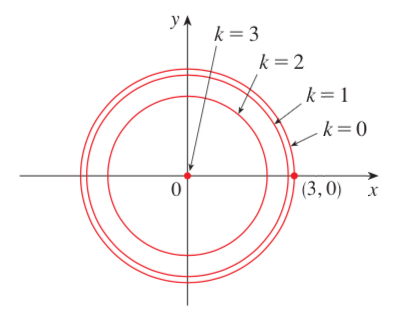
\includegraphics[scale=0.4]{../../../../img/curvasdenivel}			
		\end{center}
\end{solucion}
\item Determinar si los siguientes limites existen o no. En caso de que existan, calcule su valor
\begin{tasks}(2)
\task $\lim\limits_{(x,y) \to (0,0)} \dfrac{x^2}{x^2+y^2}$
\task $\lim\limits_{(x,y) \to (0,0)} \dfrac{5x^2y}{x^2+y^2}$
\task $\lim\limits_{(x,y) \to (0,0)} \dfrac{xy}{x^2+y^2}$
\task $\lim\limits_{(x,y) \to (0,0)} \dfrac{x^2ye^y}{x^4+y^2}$
\task $\lim\limits_{(x,y) \to (0,0)} \dfrac{sen(x^2+y^2)}{x^2+y^2}$
\task $\lim\limits_{(x,y) \to (0,0)} \dfrac{sen(xy)}{xy}$
\end{tasks}
\begin{solucion}

\begin{enumerate}[a)]
\item $\lim\limits_{(x,y) \to (0,0)} \dfrac{x^2}{x^2+y^2}$\\
			\\
			Notemos que a simple vista el grado del numerador y el denominador son iguales, por lo que es de esperarse que el límite no exista.
			
			Probemos desde distintas direcciones
			$$x = 0 \ra \lim\limits_{(0,y) \to (0,0)} \dfrac{0^2}{0^2+y^2}
			= 0$$
			$$y = 0 \ra \lim\limits_{(x,0) \to (0,0)} \dfrac{x^2}{x^2+0^2}
			= 1$$
			Como $0 \neq 1$, concluimos que el límite no existe.
\item $\lim\limits_{(x,y) \to (0,0)} \dfrac{5x^2y}{x^2+y^2}$\\
			\\
			En este caso, el grado del numerador es 3 y el del denominador es 2 por lo que, siendo el numerador mayor al denominador, es de esperarse que el límite exista (y probablemente sea igual a 0).
			
			Probemos desde distintas direcciones.
			$$x = 0 \ra \lim\limits_{(0,y) \to (0,0)} \dfrac{5\cdot0^2y}{0^2+y^2} = 0$$
			$$y = 0 \ra \lim\limits_{(x,0) \to (0,0)} \dfrac{5x^2\cdot 0}{x^2+0^2} = 0$$
			$$y = mx \ra \lim\limits_{(x,mx) \to (0,0)} \dfrac{5x^2 mx}{x^2+(mx)^2}
			= \lim\limits_{(x,mx) \to (0,0)} \dfrac{5mx^3}{x^2+m^2x^2}$$
			$$\qquad \quad = \lim\limits_{(x,mx) \to (0,0)} \dfrac{5mx^3}{x^2(1+m^2)}
			= \lim\limits_{(x,mx) \to (0,0)} \dfrac{5mx}{1+m^2}$$
			$$= \dfrac{0}{1+m^2} = 0$$
			Hasta el momento todo indica que el límite existe, sin embargo, para estar seguros es necesario comprobar con coordenadas polares, por lo que haremos el cambio de variables
			$$x = rcos(\theta), \quad y = rsen(\theta)$$
			Notemos que con este cambio,
			$$x^2+y^2 = r^2, \quad (x,y)\ra 0 \Longrightarrow r \ra 0$$
			Luego, debemos resolver el límite
			$$\lim\limits_{r\ra 0} \dfrac{5r^2cos^2(\theta)rsen(\theta)}{r^2}
			= \lim\limits_{r\ra 0} 5rcos^2(\theta)sen(\theta) = 0$$
			Como las funciones $sen$ y $cos$ son funciones acotadas, por teorema del sandwich concluimos que el límite existe y es cero.
\item $\lim\limits_{(x,y) \to (0,0)} \dfrac{xy}{x^2+y^2}$\\
			\\
			En este caso, el grado del numerador y el denominador son iguales, por lo que es de esperarse que el límite no exista.
			
			Probemos desde distintas direcciones.
			$$x = 0 \ra \lim\limits_{(0,y) \to (0,0)} \dfrac{0\cdot y}{0^2+y^2} = 0$$
			$$y = 0 \ra \lim\limits_{(x,0) \to (0,0)} \dfrac{x\cdot 0}{x^2+0^2} = 0$$
			$$y = mx \ra \lim\limits_{(x,mx) \to (0,0)} \dfrac{x mx}{x^2+(mx)^2}
			= \lim\limits_{(x,mx) \to (0,0)} \dfrac{mx^2}{x^2+m^2x^2}$$
			$$ = \lim\limits_{(x,mx) \to (0,0)} \dfrac{mx^2}{x^2(1+m^2)}
			= \dfrac{m}{1+m^2}$$
			Como el resultado depende de $m$, para distintos valores de $m$ el valor será distinto, por lo que concluimos que el límite no existe.
\item $\lim\limits_{(x,y) \to (0,0)} \dfrac{x^2ye^y}{x^4+y^2}$\\
			\\
			A simple vista, el grado del numerador es 3 y el del denominador es 4 por lo que, dado que el numerador es menor que el denominador, es de esperarse que el límite no exista.
			
			Probemos desde distintas direcciones.
			$$x = 0 \ra \lim\limits_{(0,y) \to (0,0)} \dfrac{0^2ye^y}{0^4+y^2} = 0$$
			$$y = 0 \ra \lim\limits_{(x,0) \to (0,0)} \dfrac{x^2\cdot \cdot e^0}{x^4+0^2} = 0$$
			$$y = mx \ra \lim\limits_{(x,mx) \to (0,0)} \dfrac{mx^3e^{mx}}{x^4+m^2x^2} = 
			\lim\limits_{(x,mx) \to (0,0)} \dfrac{mxe^{mx}}{x^2+m^2} = 0$$
			Hasta el momento todo indica que el límite si existe y es cero, sin embargo, como intuitivamente dijimos que no debía existir, busquemos otro acercamiento al límite. Notemos que el exponente del $x$ y el $y$ en el denominador son $4$ y $2$, respectivamente, por lo que probaremos con una función que iguale estos exponente. Esta puede ser, cualquiera de la forma $y = mx^2$.
			$$y = mx^2 \ra \lim\limits_{(x,mx^2) \to (0,0)} \dfrac{mx^4e^{mx^2}}{x^4+m^2x^4} = 
			\lim\limits_{(x,mx) \to (0,0)} \dfrac{me^{mx^2}}{1+m^2} = \dfrac{m}{1+m^2} \neq 0$$
			Finalmente, concluimos que el límite no existe.
\item $\lim\limits_{(x,y) \to (0,0)} \dfrac{sen(x^2+y^2)}{x^2+y^2}$\\
\\
Probemos desde distintas direcciones.
$$x = 0 \ra \lim\limits_{(0,y) \to (0,0)} \dfrac{sen(0^2+y^2)}{0^2+y^2} 
= \lim\limits_{y \to 0} \dfrac{sen(y^2)}{y^2}
= 1$$
$$y = 0 \ra \lim\limits_{(x,0) \to (0,0)} \dfrac{sen(x^2+0^2)}{x^2+0^2} 
= \lim\limits_{x \to 0} \dfrac{sen(x^2)}{x^2}
= 1$$
$$y = mx \ra \lim\limits_{(x,mx) \to (0,0)} \dfrac{sen(x^2+(mx)^2)}{x^2+(mx)^2} 
= \lim\limits_{x \to 0} \dfrac{sen(x^2(1+m^2))}{x^2(1+m^2)}
= 1$$
Ahora, comprobamos en polares
$$x = rcos(\theta), \quad y = rsen(\theta)$$
$$x^2 + y^2 = r^2$$
Con esto, el límite queda
$$\lim\limits_{r\ra 0} \dfrac{sen(r^2)}{r^2} = 1$$
\item $\lim\limits_{(x,y) \to (0,0)} \dfrac{sen(xy)}{xy}$\\
\\
Probemos directamente con polares,
$$x = rcos(\theta), \quad y = rsen(\theta)$$
Con esto, el límite queda
$$\lim\limits_{r\ra 0} \dfrac{sen(rcos(\theta) rsen(\theta))}{rcos(\theta) rsen(\theta)}$$
Uno tendería a pensar que esto es 1, sin embargo, si evaluamos con $\theta = 0$ antes de evaluar $r$, nos queda $\dfrac{0}{0}$, lo que es indefinido. Ojo que esto no es lo mismo que un límite que al evaluarlo nos queda $\dfrac{0}{0}$, ya que eso sería $\dfrac{casi\ 0}{casi\ 0}$. Aquí lo que ocurre es un real $\dfrac{0}{0}$, cosa que es imposible.\\

Por lo tanto, el límite no existe.\\

Como conclusión, para que el límite exista, este debe ser igual para cualquier valor de $\theta$, incluso antes de evaluar el límite.
\end{enumerate}
\end{solucion}
\item Dada la función 
	$$ f(x) = 
	\begin{cases}
	\dfrac{x^4y^3}{3x^2+2y^2} & si\ (x,y) \neq (0,0) \\
	0 & si\ (x,y) = (0,0)
	\end{cases}
	$$
	determinar si es continua en todo $\R^2$ o no.
\begin{solucion}
Para que la función sea continua debe ocurrir que 
$$\lim\limits_{(x,y) \to (0,0)} f(x,y) = f(0,0) = 0$$

$\lim\limits_{(x,y) \to (0,0)} \dfrac{5x^2y}{x^2+y^2}$\\
			\\
			En este caso, el grado del numerador es 3 y el del denominador es 2 por lo que, siendo el numerador mayor al denominador, es de esperarse que el límite exista (y probablemente sea igual a 0).
			
			Probemos desde distintas direcciones.
$$x = 0 \ra \lim\limits_{(0,y) \to (0,0)} \dfrac{0^4y^3}{3\cdot0^2+2y^2} = 0$$
$$y = 0 \ra \lim\limits_{(x,0) \to (0,0)} \dfrac{x^40^3}{3x^2+2\cdot 0^2} = 0$$
$$y = mx \ra \lim\limits_{(x,mx) \to (0,0)} \dfrac{x^4 (mx)^3}{3x^2+2m^2x^2}
= \lim\limits_{(x,mx) \to (0,0)} \dfrac{m^3x^7}{x^2(3+2m^2)}
= \lim\limits_{(x,mx) \to (0,0)} \dfrac{m^3x^5}{3+2m^2} = 0$$
			Hasta el momento todo indica que el límite existe, sin embargo, para estar seguros es necesario comprobar con coordenadas polares, por lo que haremos el cambio de variables
$$x = \sqrt[]{2}rcos(\theta), \quad y = \sqrt[]{3}rsen(\theta)$$
Notemos que con este cambio,
$$3x^2+2y^2 = 6r^2, \quad (x,y)\ra 0 \Longrightarrow r \ra 0$$
Luego, debemos resolver el límite
$$\lim\limits_{r\ra 0} \dfrac{r^4cos^4(\theta)r^3sen^3(\theta)}{6r^2}
			= \lim\limits_{r\ra 0} \dfrac{1}{6}r^5cos^4(\theta)sen^3(\theta) = 0$$
			Como las funciones $sen$ y $cos$ son funciones acotadas, por teorema del sandwich concluimos que el límite existe y es cero.\\
\\
Finalmente, la función es continua.
\end{solucion}
\item Determine el conjunto de puntos en los cuales la función es continua
	$$f(x,y) = 
	\begin{cases}
	\dfrac{x^3y^2}{x^2+2y^2} & (x,y) \neq (0,0)\\
	1 & (x,y) = (0,0)
	\end{cases}
	$$
\begin{solucion}
Notemos que para todo $(x,y) \neq (0,0)$, $f(x,y)$ es continua por ser composición de funciones continuas.\\

Luego, solo nos queda ver que ocurre en $(0,0)$.\\

Para que la función sea continua en $(0,0)$ debe ocurrir que 
$$\lim\limits_{(x,y) \to (0,0)} f(x,y) = f(0,0) = 1$$
			
			Probemos desde distintas direcciones.
$$x = 0 \ra \lim\limits_{(0,y) \to (0,0)} \dfrac{0^3y^2}{0^2+2y^2} = 0$$
$$y = 0 \ra \lim\limits_{(x,0) \to (0,0)} \dfrac{x^30^2}{x^2+2\cdot 0^2} = 0$$
$$y = mx \ra \lim\limits_{(x,mx) \to (0,0)} \dfrac{x^3 (mx)^2}{x^2+2m^2x^2}
= \lim\limits_{(x,mx) \to (0,0)} \dfrac{m^2x^5}{x^2(1+2m^2)}
= \lim\limits_{(x,mx) \to (0,0)} \dfrac{m^2x^3}{1+2m^2} = 0$$
			Hasta el momento todo indica que el límite existe, sin embargo, para estar seguros es necesario comprobar con coordenadas polares, por lo que haremos el cambio de variables
$$x = rcos(\theta), \quad y = \sqrt[]{2}rsen(\theta)$$
Notemos que con este cambio,
$$2x^2+y^2 = 2r^2, \quad (x,y)\ra 0 \Longrightarrow r \ra 0$$
Luego, debemos resolver el límite
$$\lim\limits_{r\ra 0} \dfrac{r^3cos^3(\theta)r^2sen^2(\theta)}{2r^2}
			= \lim\limits_{r\ra 0} \dfrac{1}{2}r^3cos^3(\theta)sen^2(\theta) = 0$$
			Como las funciones $sen$ y $cos$ son funciones acotadas, por teorema del sandwich concluimos que el límite existe y es cero.\\
\\
Por lo tanto, la función es continua en $\R^2 - (0,0)$.
\end{solucion}
\item Determine la derivada por definición en $x$ de la función
	$$f(x,y) = 2xy + x^2y + x + y$$
\begin{solucion}
Para determinar la derivada en $x$ debemos resolver el siguiente límite
		$$f_x = \lim\limits_{h \ra 0} \dfrac{f(x+h,y) - f(x,y)}{h}$$
		En nuestro caso,
		$$f_x = \lim\limits_{h \ra 0} \dfrac{2(x+h)y + (x+h)^2y + (x+h) + y - (2xy + x^2y + x + y)}{h}$$
		$$= \lim\limits_{h \ra 0} \dfrac{2xy+2hy + x^2y+2xhy + yh^2 + x+h + y - 2xy - x^2y - x - y}{h}$$
		$$= \lim\limits_{h \ra 0} \dfrac{2hy+2xhy + h^2 +h}{h}
		= \lim\limits_{h \ra 0} \dfrac{h(2y+2xy + hy +1)}{h}$$
		$$= \lim\limits_{h \ra 0} 2y+2xy + hy +1
		= 2y+2xy+1$$
\end{solucion}
\item Para las siguientes funciones, calcular $f_x$ y $f_y$
\begin{enumerate}[a)]
\item $f(x,y) = \dfrac{xy}{x-y}$
\item $f(x,y) = (x^2+y^2)sen\left(\dfrac{1}{x^2+y^2}\right)$
\end{enumerate}
\begin{solucion}

\begin{enumerate}[a)]
\item $f(x,y) = \dfrac{xy}{x-y}$\\
			\\
			$$f_x = \dfrac{y(x-y)-xy}{(x-y)^2} = -\dfrac{y^2}{(x-y)^2}$$
			$$f_y = \dfrac{x(x-y)+xy}{(x-y)^2} = \dfrac{x^2}{(x-y)^2}$$
\item $f(x,y) = (x^2+y^2)sen\left(\dfrac{1}{x^2+y^2}\right)$
			$$f_x = 2x\ sen\left(\dfrac{1}{x^2+y^2}\right) + cos\left(\dfrac{1}{x^2+y^2}\right) \cdot \dfrac{-1}{(x^2+y^2)^2} \cdot 2x \cdot (x^2+y^2)$$
			$$ = 2x\ sen\left(\dfrac{1}{x^2+y^2}\right) - cos\left(\dfrac{1}{x^2+y^2}\right) \cdot \dfrac{2x}{x^2+y^2}$$
			$$f_y = 2x\ sen\left(\dfrac{1}{x^2+y^2}\right) + cos\left(\dfrac{1}{x^2+y^2}\right) \cdot \dfrac{-1}{(x^2+y^2)^2} \cdot 2y \cdot (x^2+y^2)$$
			$$ = 2x\ sen\left(\dfrac{1}{x^2+y^2}\right) - cos\left(\dfrac{1}{x^2+y^2}\right) \cdot \dfrac{2y}{x^2+y^2}$$
			Notemos que ambas derivadas son practicamente iguales, pero se cambiando de lugar las variables. Esto es porque la función cumple que $f(x,y) = f(y,x)$
\end{enumerate}
\end{solucion}
\item Una función armónica es aquella que cumple con $f_{xx} + f_{yy} = 0$. Determina si la siguiente funcion es armónica
	$$f(x,y) = xy + 3x^2 -y^3$$
\begin{solucion}
Derivando,
		$$f_x = y + 6x \ra f_{xx} = 6$$
		$$f_y = x -3y^2 \ra f_{yy} = -6y$$
		Como $f_{xx} + f_{yy} = 6 - 6y \neq 0$, concluimos que la función no es armónica.
\end{solucion}
\item Busque $\dfrac{\delta z}{\delta t}$ o $\dfrac{\delta w}{\delta t}$, según corresponda.
\begin{enumerate}[a)]
\item $z = x^2+y^2+xy$\tab$x=sen(t), y=e^t$
\item $w=xe^{y/z}$\tab$x=t^2, y=1-t, z=1+2t$
\item $w=ln(\sqrt[]{x^2+y^2+z^2})$\tab$x=sen(t), y=cos(t), z=tan(t)$
\end{enumerate}
\begin{solucion}

\begin{enumerate}[a)]
\item $z = x^2+y^2+xy$\tab$x=sen(t), y=e^t$\\
			\\
			$z_t = z_x x_t + z_y y_z = (2x+y)cos(t) + (2y+x)e^t$
\item $w=xe^{y/z}$\tab$x=t^2, y=1-t, z=1+2t$\\
			\\
			{\small$w_t = w_x x_t + w_y y_t + w_z z_t = e^{y/z} 2t + xe^{y/z}\dfrac{1}{z}\cdot(-1) + xe^{y/z} \cdot \dfrac{-1}{z^2}\cdot 2 = e^{y/z}\left(2t - \dfrac{x}{z} - \dfrac{2x}{z^2}\right)$}
\item $w=ln(\sqrt[]{x^2+y^2+z^2})$\tab$x=sen(t), y=cos(t), z=tan(t)$\\
			\\
			$w_t = w_x x_t + w_y y_t + w_z z_t$
			$$ = \dfrac{1}{\sqrt[]{x^2+y^2+z^2}}\cdot \dfrac{1}{2\ \sqrt[]{x^2+y^2+z^2}} (2x\ cos(t) - 2y\ sen(t) + 2z\ sec^2(t))$$
			$$ = \dfrac{1}{x^2+y^2+z^2} (x\ cos(t) - y\ sen(t) + z\ sec^2(t)) \qquad \qquad \qquad \qquad \qquad$$
\end{enumerate}
\end{solucion}
\item Sea $f$ una función con segundas derivadas parciales continuas en todo $R^2$. El cambio de variables $x=uv$, $y=\dfrac{u^2-v^2}{2}$ transforma la función $f(x,y)$ en la función $g(u,v)$.
\begin{enumerate}[a)]
\item Calcule $\dfrac{\delta g}{\delta u}, \dfrac{\delta g}{\delta v}$ en terminos de las derivadas parciales de $f$.
\item Si $f_{xx}(x,y) + f_{yy}(x,y) = 2$ para todo $(x,y) \in R^2$, determine las constantes $a,b \in \R$ tales que
		$$a\dfrac{\delta^2g}{\delta u^2} - b\dfrac{\delta^2 g}{\delta v^2} = u^2 + v^2$$
\end{enumerate}
\begin{solucion}
Antes de comenzar, calculemos las derivadas parciales de $x$ e $y$, ya que las usaremos varias veces, esto es
	$$x_u = v,\quad  x_v = u,\quad y_u = u, \quad y_v = -v$$
\begin{enumerate}[a)]
\item Calcule $\dfrac{\delta g}{\delta u}, \dfrac{\delta g}{\delta v}$ en terminos de las derivadas parciales de $f$.\\
\\
Notemos que lo que nos están pidiendo es equivalente a calcular $f_u$ y $f_v$.
$$f_u = f_x x_u + f_y y_u = f_x v + f_y u $$
$$f_v = f_x x_v + f_y y_v = f_x u - f_y v $$
\item Si $f_{xx}(x,y) + f_{yy}(x,y) = 2$ para todo $(x,y) \in R^2$, determine las constantes $a,b \in \R$ tales que
$$a\dfrac{\delta^2g}{\delta u^2} - b\dfrac{\delta^2 g}{\delta v^2} = u^2 + v^2$$\\
\\
En primer lugar, debemos calcular $f_{uu}$ y $f_{vv}$.\\

Comencemos por $f_{uu}$, esto es
$$f_{uu} = (f_u)_u = (f_x v + f_y u)_u =(f_x v)_u + (f_y u)_u$$
Veamos estos terminos por separado.\\
\\
En primer lugar, $(f_x v)_u$. Como estamos derivando en $u$, la $v$ es una constante, por lo que
$$(f_x v)_u = f_{xu}v$$
Luego, debemos derivar $f_x$ en $u$. Como $f_x$ es una función que depende de $x$ e $y$, también debemos aplicar la regla de la cadena, esto es,
$$v f_{xu} = (f_{xx} x_u + f_{xy} y_u)v = (f_{xx} v + f_{xy} u)v $$
Ahora, veamos que ocurre con $(f_y u)_u$. En este caso, $f_y$ esta multiplicado por $u$. Como estamos derivando en la variable $u$, esto ya no es una constante, por lo que debemos aplicar la regla de la multiplicación. Luego,
$$(f_y u)_u =  f_{yu}u + f_y = (f_{yx} x_u + f_{yy} y_u)u + f_y =  (f_{yx} v + f_{yy} u)u + f_y$$
Por lo tanto,
$$f_{uu} = (f_{xx} v + f_{xy} u)v + (f_{yx} v + f_{yy} u)u + f_y$$
Además, por el Teorema de Clairaut, sabemos que $f_{xy} = f_{yx}$\\
\\
Simplificando,
$$f_{uu} = f_{xx}v^2 + 2f_{xy}uv + f_{yy}u^2+ f_y$$
De manera análoga, podemos ver que
$$f_{vv} = (f_x u - f_y v)_v = (f_x u)_v - (f_y v)_v$$
Luego,
$$f_{vv} = (f_{xx}x_v + f_{xy} y_v)u + - (f_{yx} x_v + f_{yy} y_v)v - f_y$$
Reemplazando,
$$f_{vv} = (f_{xx}u + f_{xy} (-v))u + - (f_{yx} u + f_{yy} (-v))v - f_y$$
Simplificando,
$$f_{vv} = f_{xx}u^2 - 2f_{xy}uv + f_{yy}v^2 + f_y$$
Ahora que tenemos $f_{uu}$ y $f_{vv}$, debemos buscar $a$ y $b$ tal que
$$af_{uu} - bf_{vv} = u^2 + v^2$$
Reemplazando,
$$a((f_{xx} v + f_{xy} u)v + (f_{yx} v + f_{yy} u)u + f_y) - b (f_{xx}u^2 - 2f_{xy}uv + f_{yy}v^2 + f_y) = u^2 + v^2$$
Reordenando, según las potencias de $u$ y $v$, tenemos
$$u^2(af_{yy} - bf_{xx}) + v^2(af_{xx} - bf_{yy}) + (a+b)(2f_{xy}uv + f_y) = u^2 + v^2$$
En primer lugar, notemos que el tercer termino debe desaparecer, por lo que necesariamente
$$a + b = 0 \ra a = -b$$
Reemplazando esto, tenemos
$$u^2(af_{yy} +af_{xx}) + v^2(af_{xx} +af_{yy}) = u^2 + v^2$$
$$u^2a(f_{yy} +f_{xx}) + v^2a(f_{xx} +f_{yy}) = u^2 + v^2$$
Por el enunciado, sabemos que $f_{xx} + f_{yy} = 2$, por lo que
$$u^22a + v^22a = u^2 + v^2$$
Luego,
$$2a = 1 \ra a = \dfrac{1}{2} \ra b = -\dfrac{1}{2}$$
\end{enumerate}
\end{solucion}
\end{preguntas}
\end{document}